\section{Fragmentation}

\pgfdeclareimage[width=1.0\paperwidth]{header-image}{header_images/helicopter}
\againframe<6->{framework}


\begin{frame}<2>[label=controlMaps]
    \frametitle{So Humans have no impact on fire?}
    \framesubtitle{Suppression \& Fragmentation}
    \controlsSide{limitation_map_no_supression_light}
\end{frame}

\addtocounter{framenumber}{-1}
\begin{frame}<2>[label=controlMaps]
	\frametitle{So Humans have no impact on fire?}
	\framesubtitle{Suppression \& Fragmentation}
	\controlsSide{limitation_map_light}
\end{frame}

\addtocounter{framenumber}{-1}
\begin{frame}<2>[label=controlMaps]
	\frametitle{So Humans have no impact on fire?}
	\framesubtitle{Suppression \& Fragmentation}
	\controlsSide{limitation_map_noColour}
\end{frame}

\addtocounter{framenumber}{-1}
\begin{frame}<2-4>[label=controlMaps]
	\frametitle{So Humans have no impact on fire?}
	\framesubtitle{Suppression \& Fragmentation}
	\controlsSide{limitation_map_light}
	
	\begin{textblock*}{14cm}(3.1cm,3.25cm)
		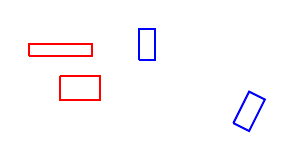
\begin{tikzpicture}
		\visible<5> {
			% Sahel
			\draw[red, line width = 0.25mm] (3.2,5.25) -- (4.0,5.25) -- (4.0,5.4) -- (3.2,5.4) -- (3.2,5.25);
			
			\draw[red, line width = 0.25mm] (3.6,5.0) -- (4.1,5.0) -- (4.1,4.7) -- (3.6,4.7) -- (3.6,5.0);
		}
		\visible<3-> {
			\draw[blue, line width = 0.25mm] (4.6,5.2) -- (4.8,5.2) -- (4.8,5.6) -- (4.6,5.6) -- (4.6,5.2);
			
			\draw[blue, line width = 0.25mm] (5.8,4.4) -- (6.0,4.3) -- (6.2,4.7) -- (6.0,4.8) -- (5.8,4.4);
		}
		\end{tikzpicture}
	\end{textblock*}
	\begin{textblock*}{14cm}(6.7cm,1.45cm)
		
		\only<3>{
			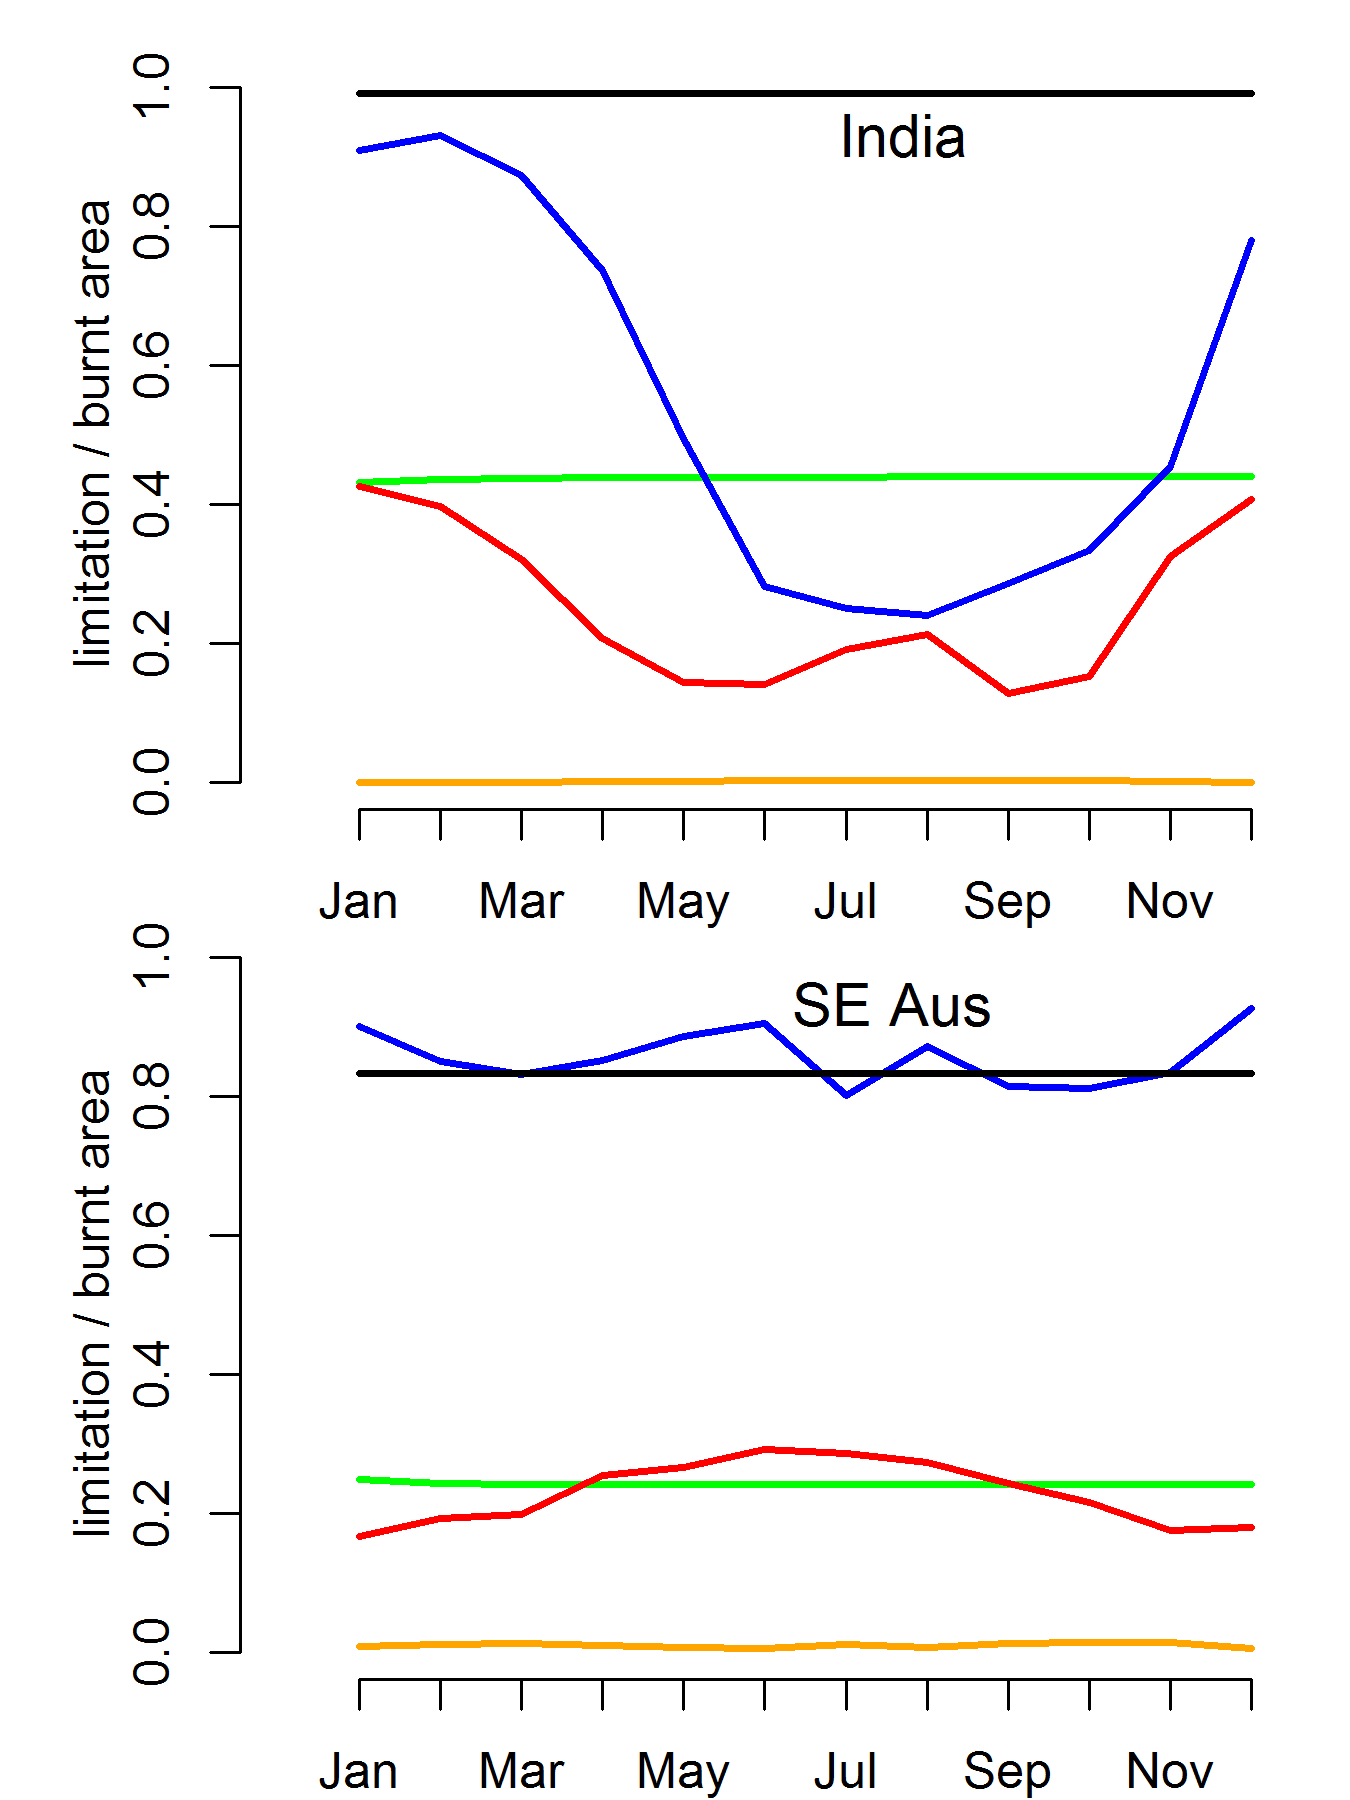
\includegraphics[width=5.7cm]{images/caseStudy/seasonal_casestudyAsia1}}
		\only<4>{
			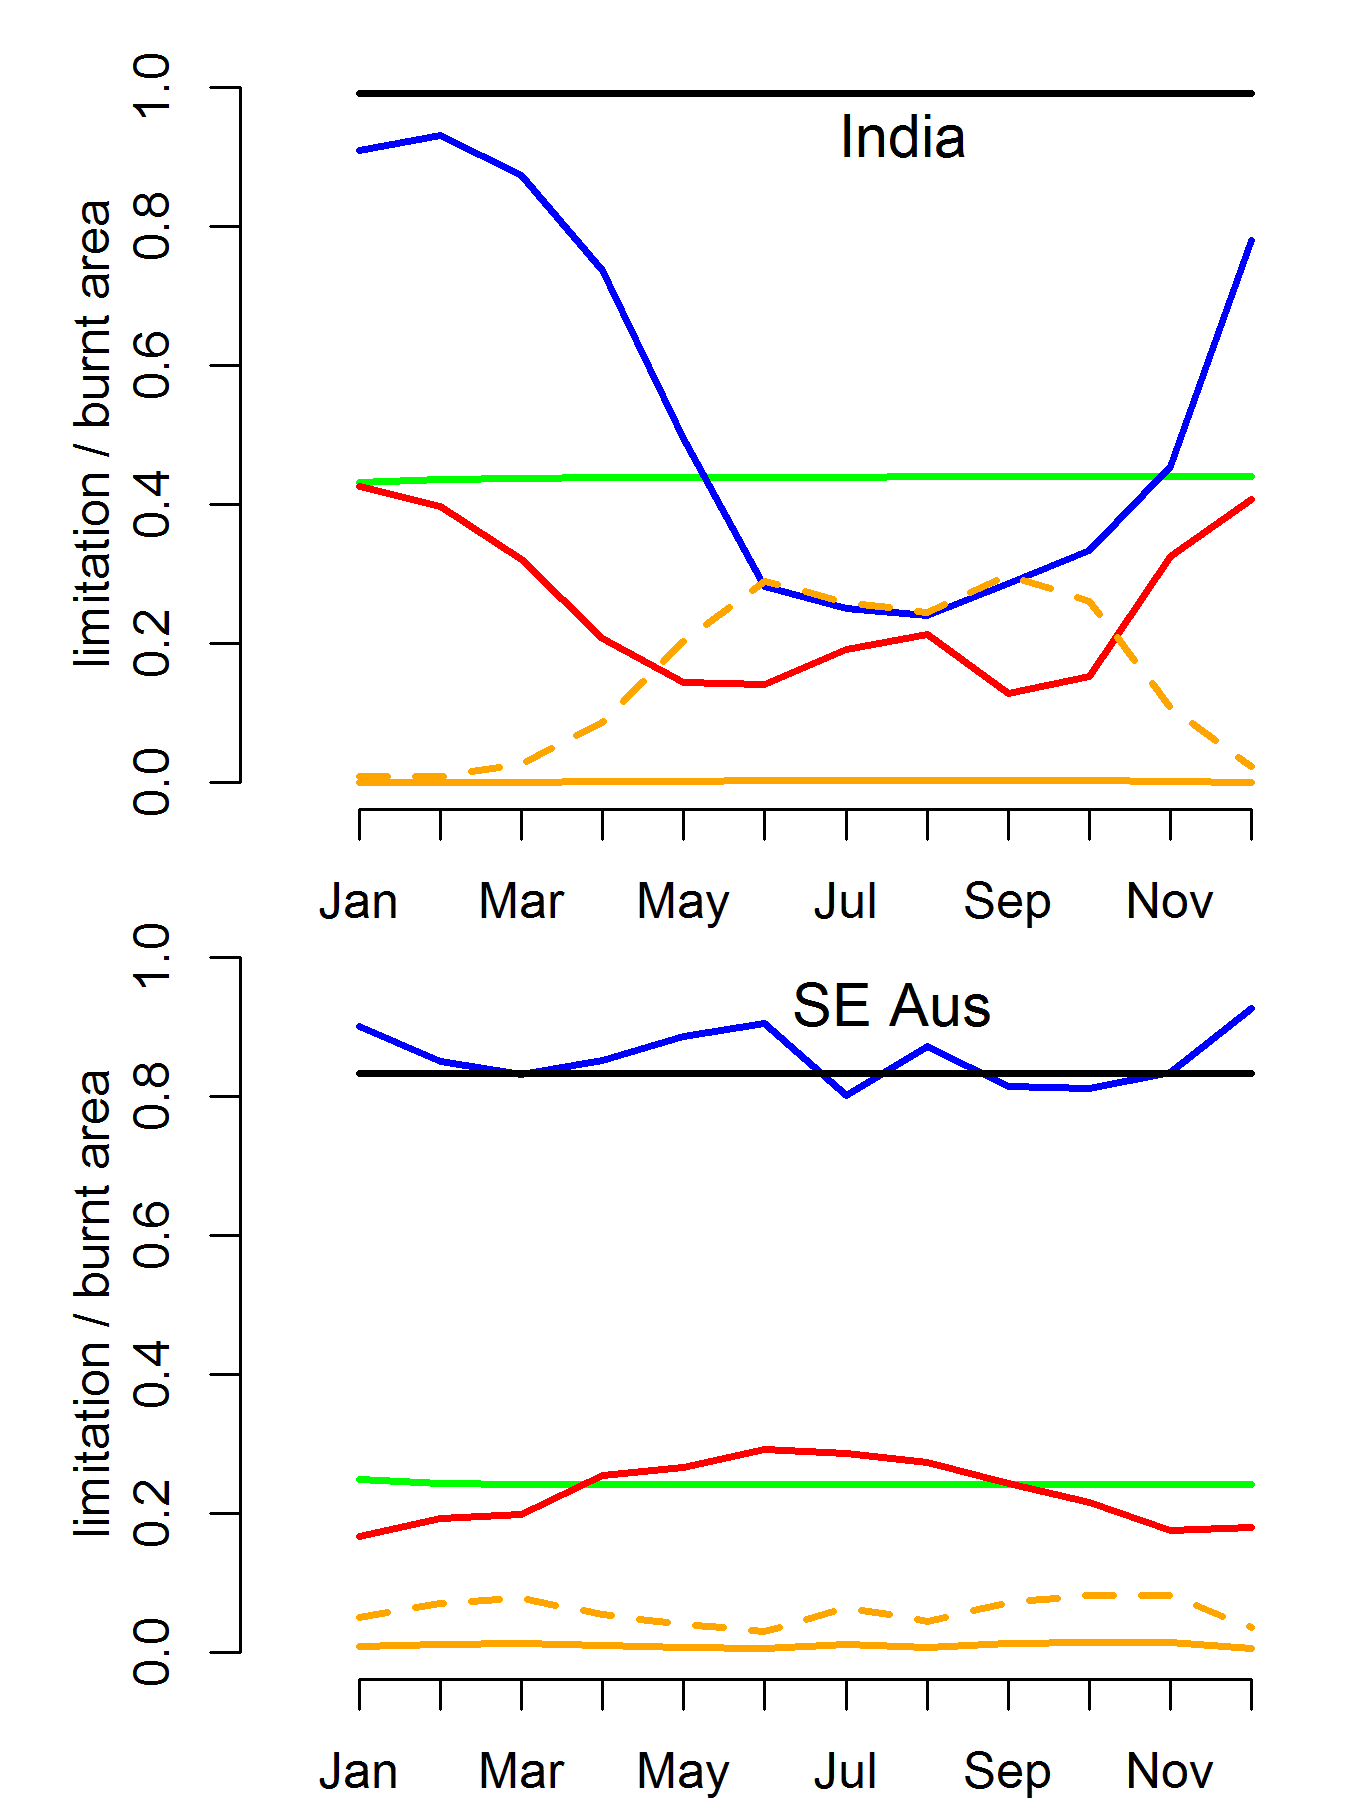
\includegraphics[width=5.7cm]{images/caseStudy/seasonal_casestudyAsia2}}
	\end{textblock*}
	
\end{frame}

\pgfdeclareimage[width=1.0\paperwidth]{header-image}{header_images/Mirador_de_Garbi}
\begin{frame}
    \frametitle{So Humans have no impact on fire?}
    \framesubtitle{Suppression \& Fragmentation}
    \begin{textblock*}{11cm}(0cm,1.5cm)
    \visible<1->{
    	\begin{tikzpicture}
    	\node[anchor=north,inner sep=0] (image) at (0,0) {
    		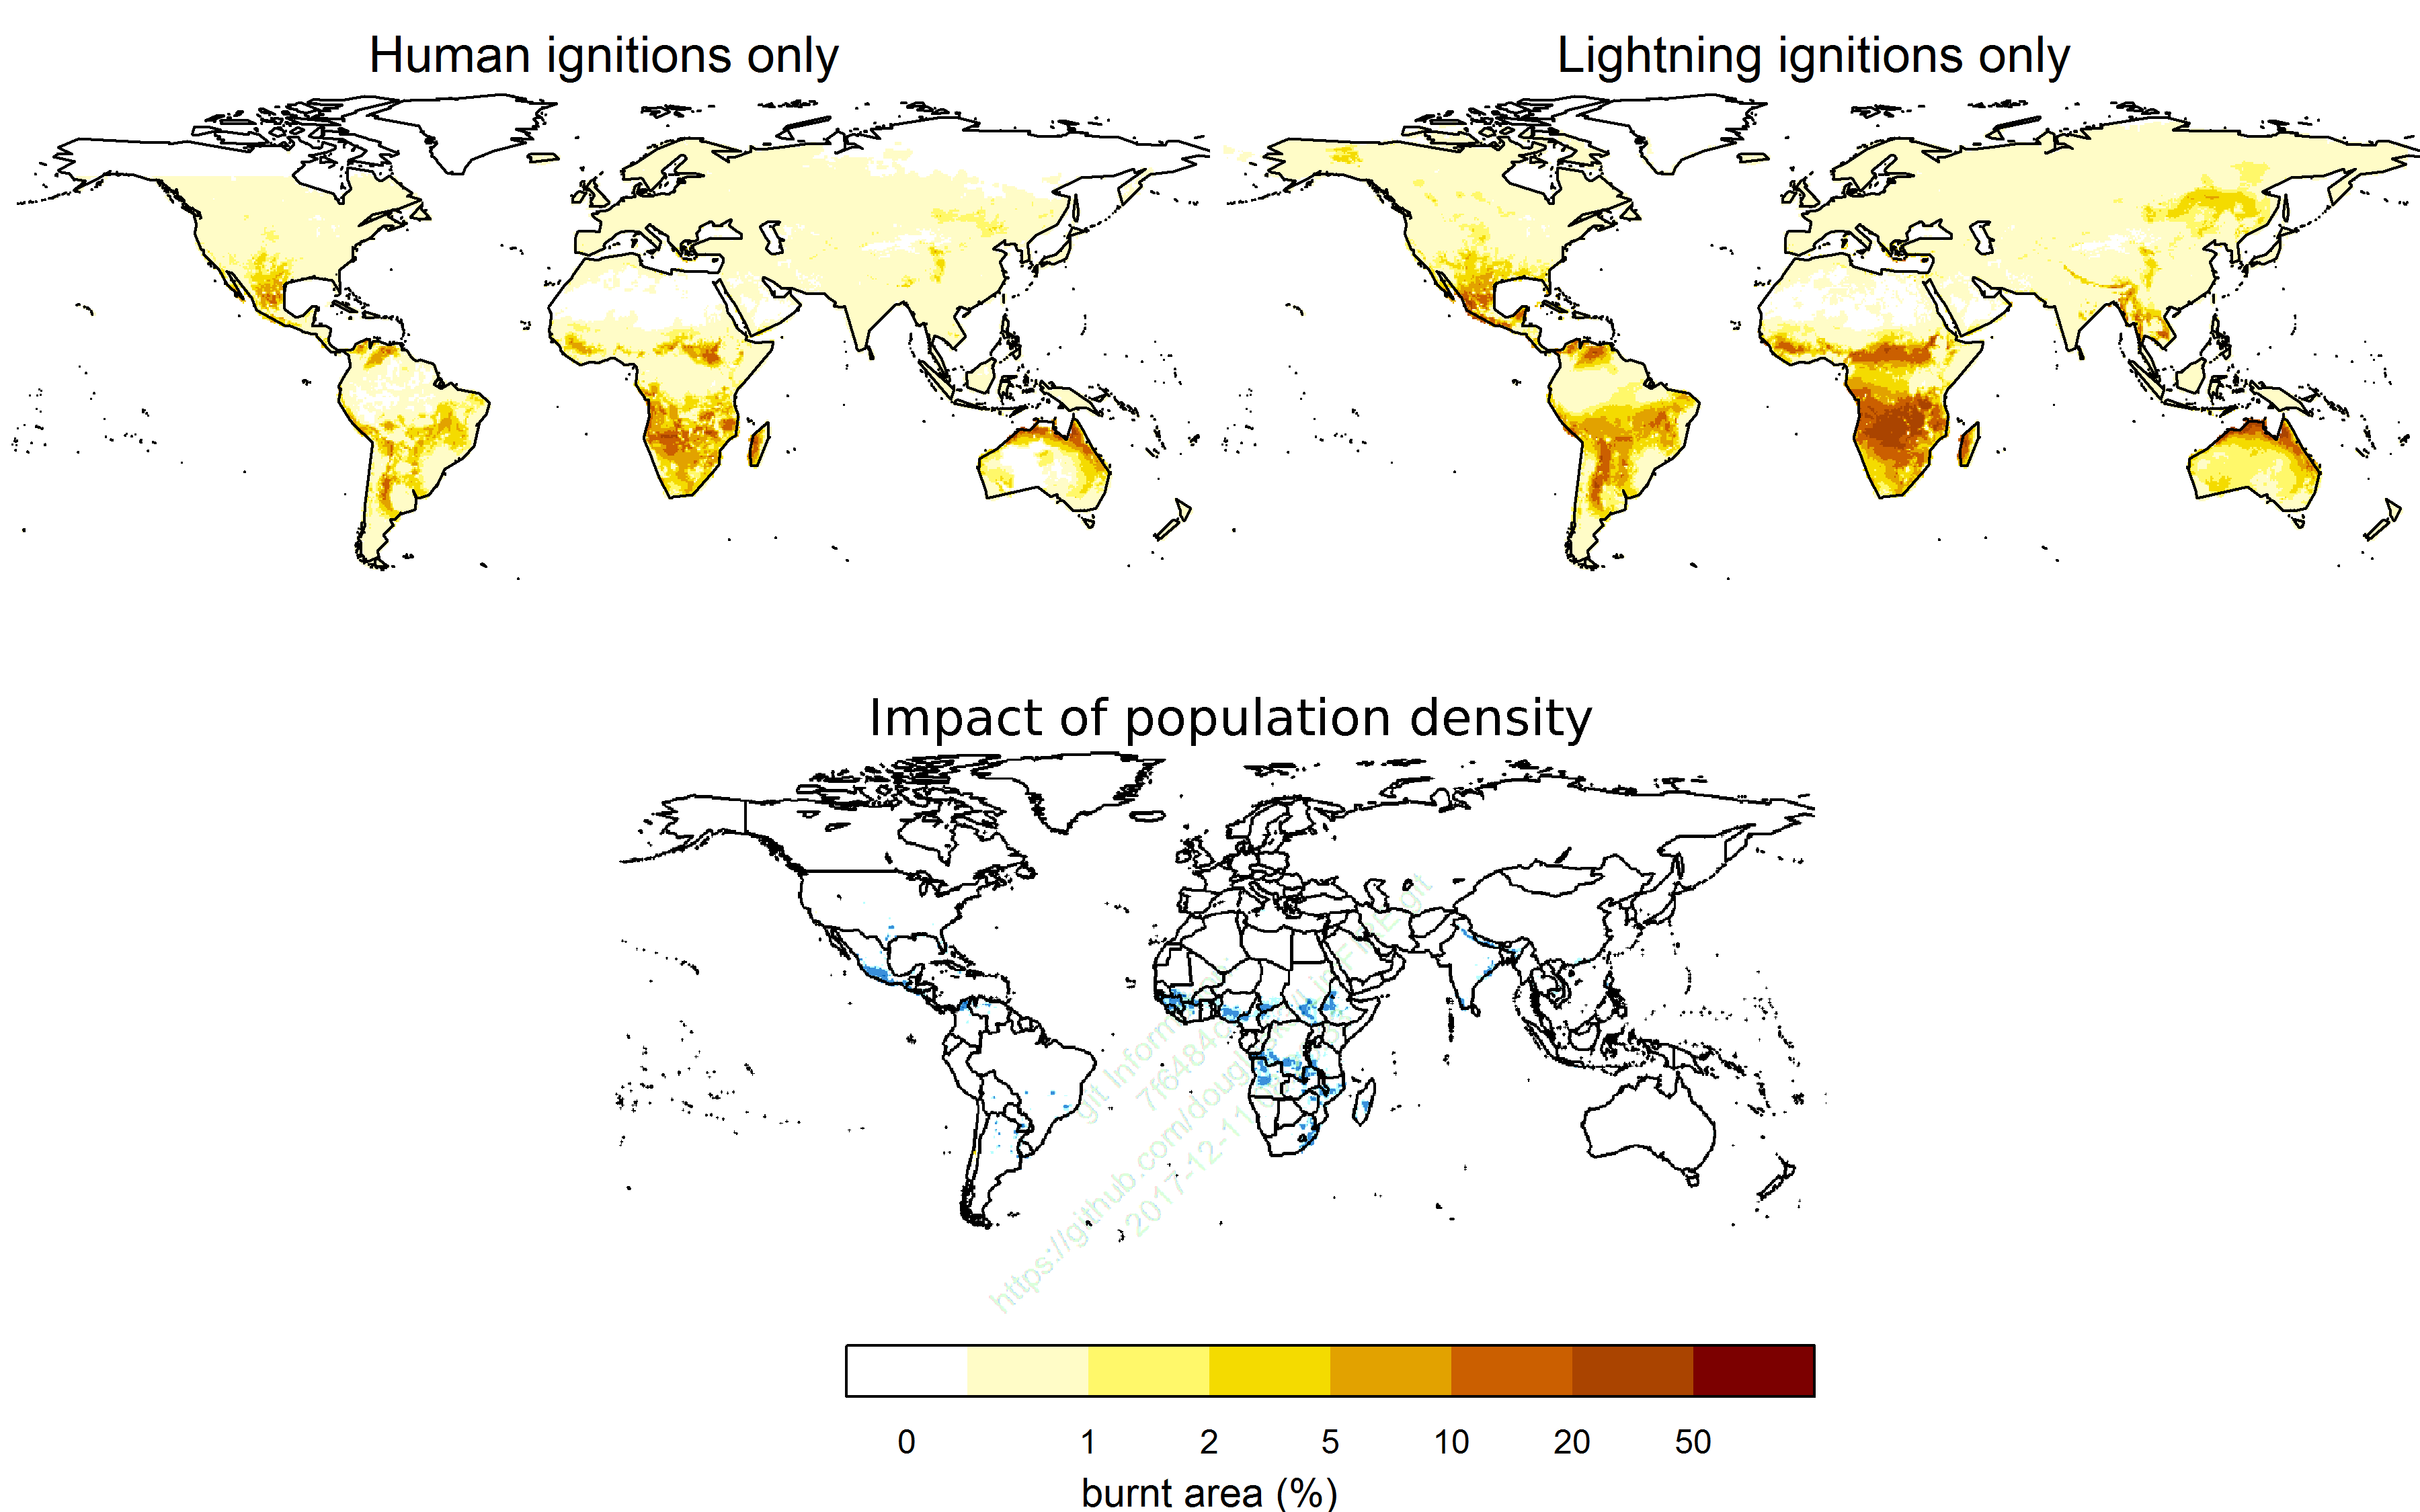
\includegraphics[trim={5.1cm 2cm 5.1cm 6.2cm},clip,width=6.2cm]{images/igntitions/IgntionInfoSourceAdding}
	    };
        \node[anchor=south,align=center] at (0, -0.2) {Human Ignitions};
        \end{tikzpicture}
    }
	%trim = {l b r t}
    \visible<1->{
    	\begin{tikzpicture}
    	\node[anchor=north,inner sep=0] (image) at (0,0) {
    		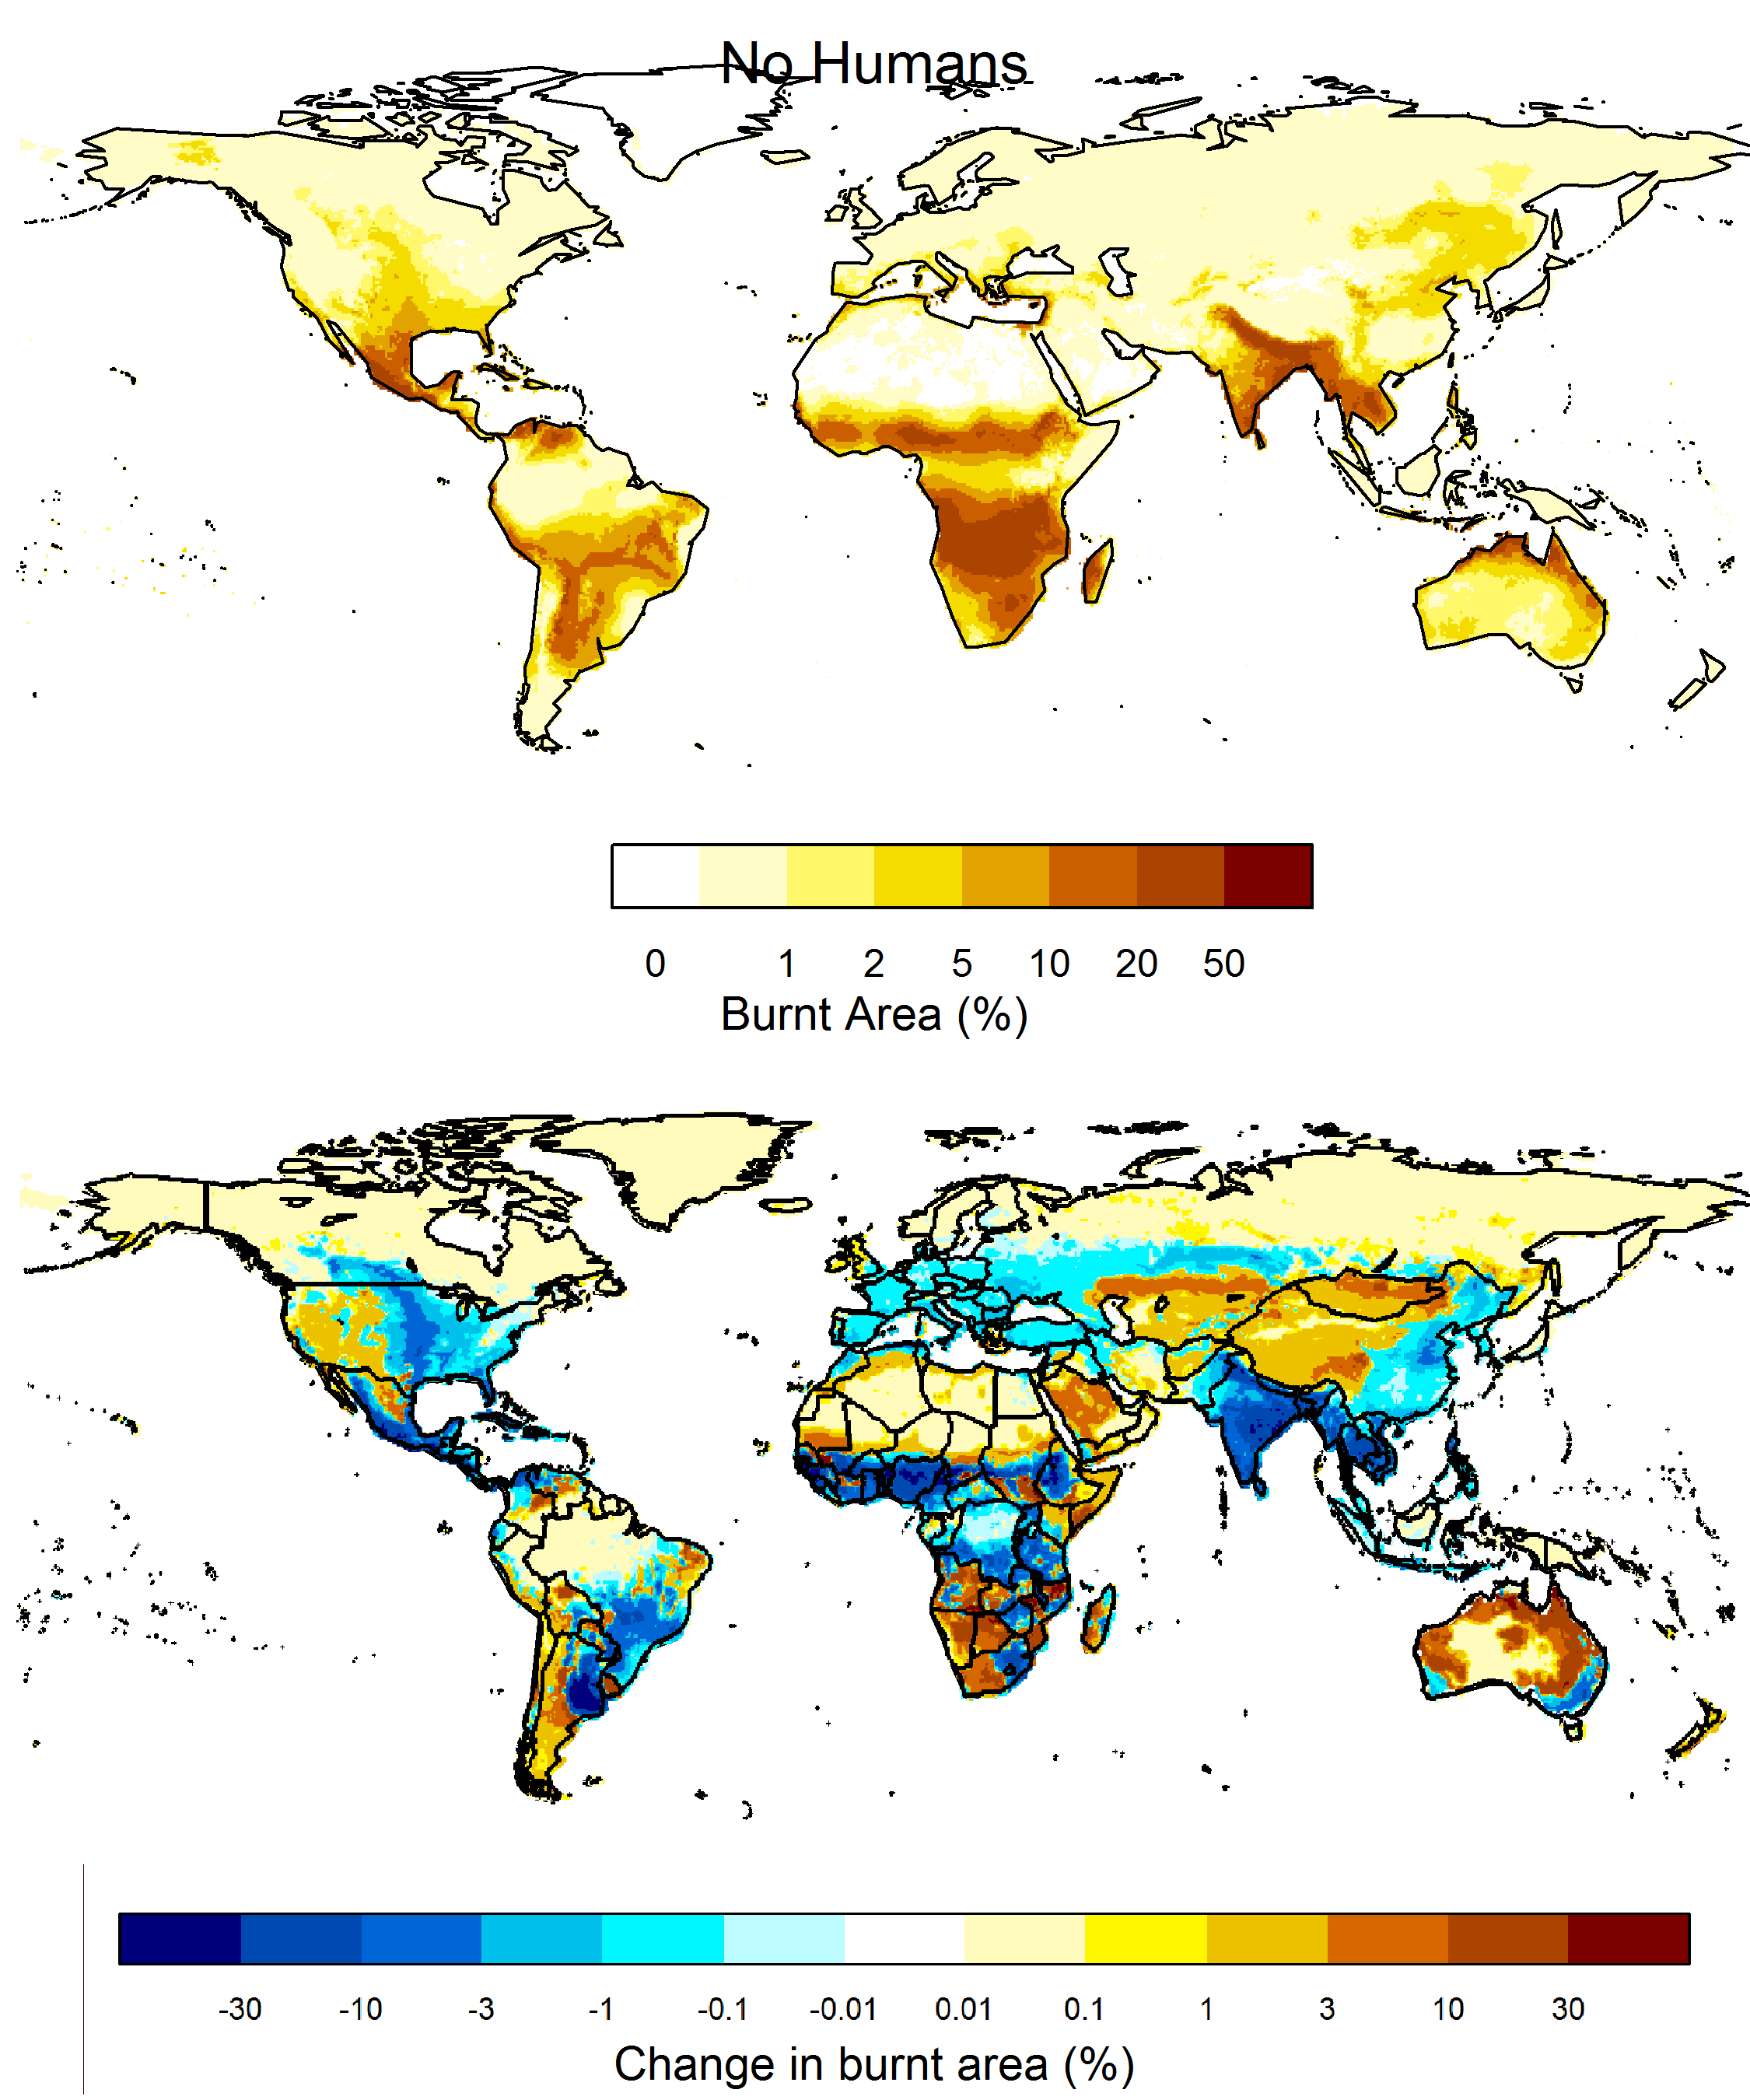
\includegraphics[trim={0 0 0 8cm},clip,width=6.2cm]{images/igntitions/IgntionInfoNoHumans}
    	};
    	\node[anchor=south,align=center] at (0, -0.2) {Overall Human Impact};
    	\end{tikzpicture}
        
    }
    \end{textblock*}
    \begin{textblock*}{11cm}(6.4cm,1.3cm)
    \visible<2->{
        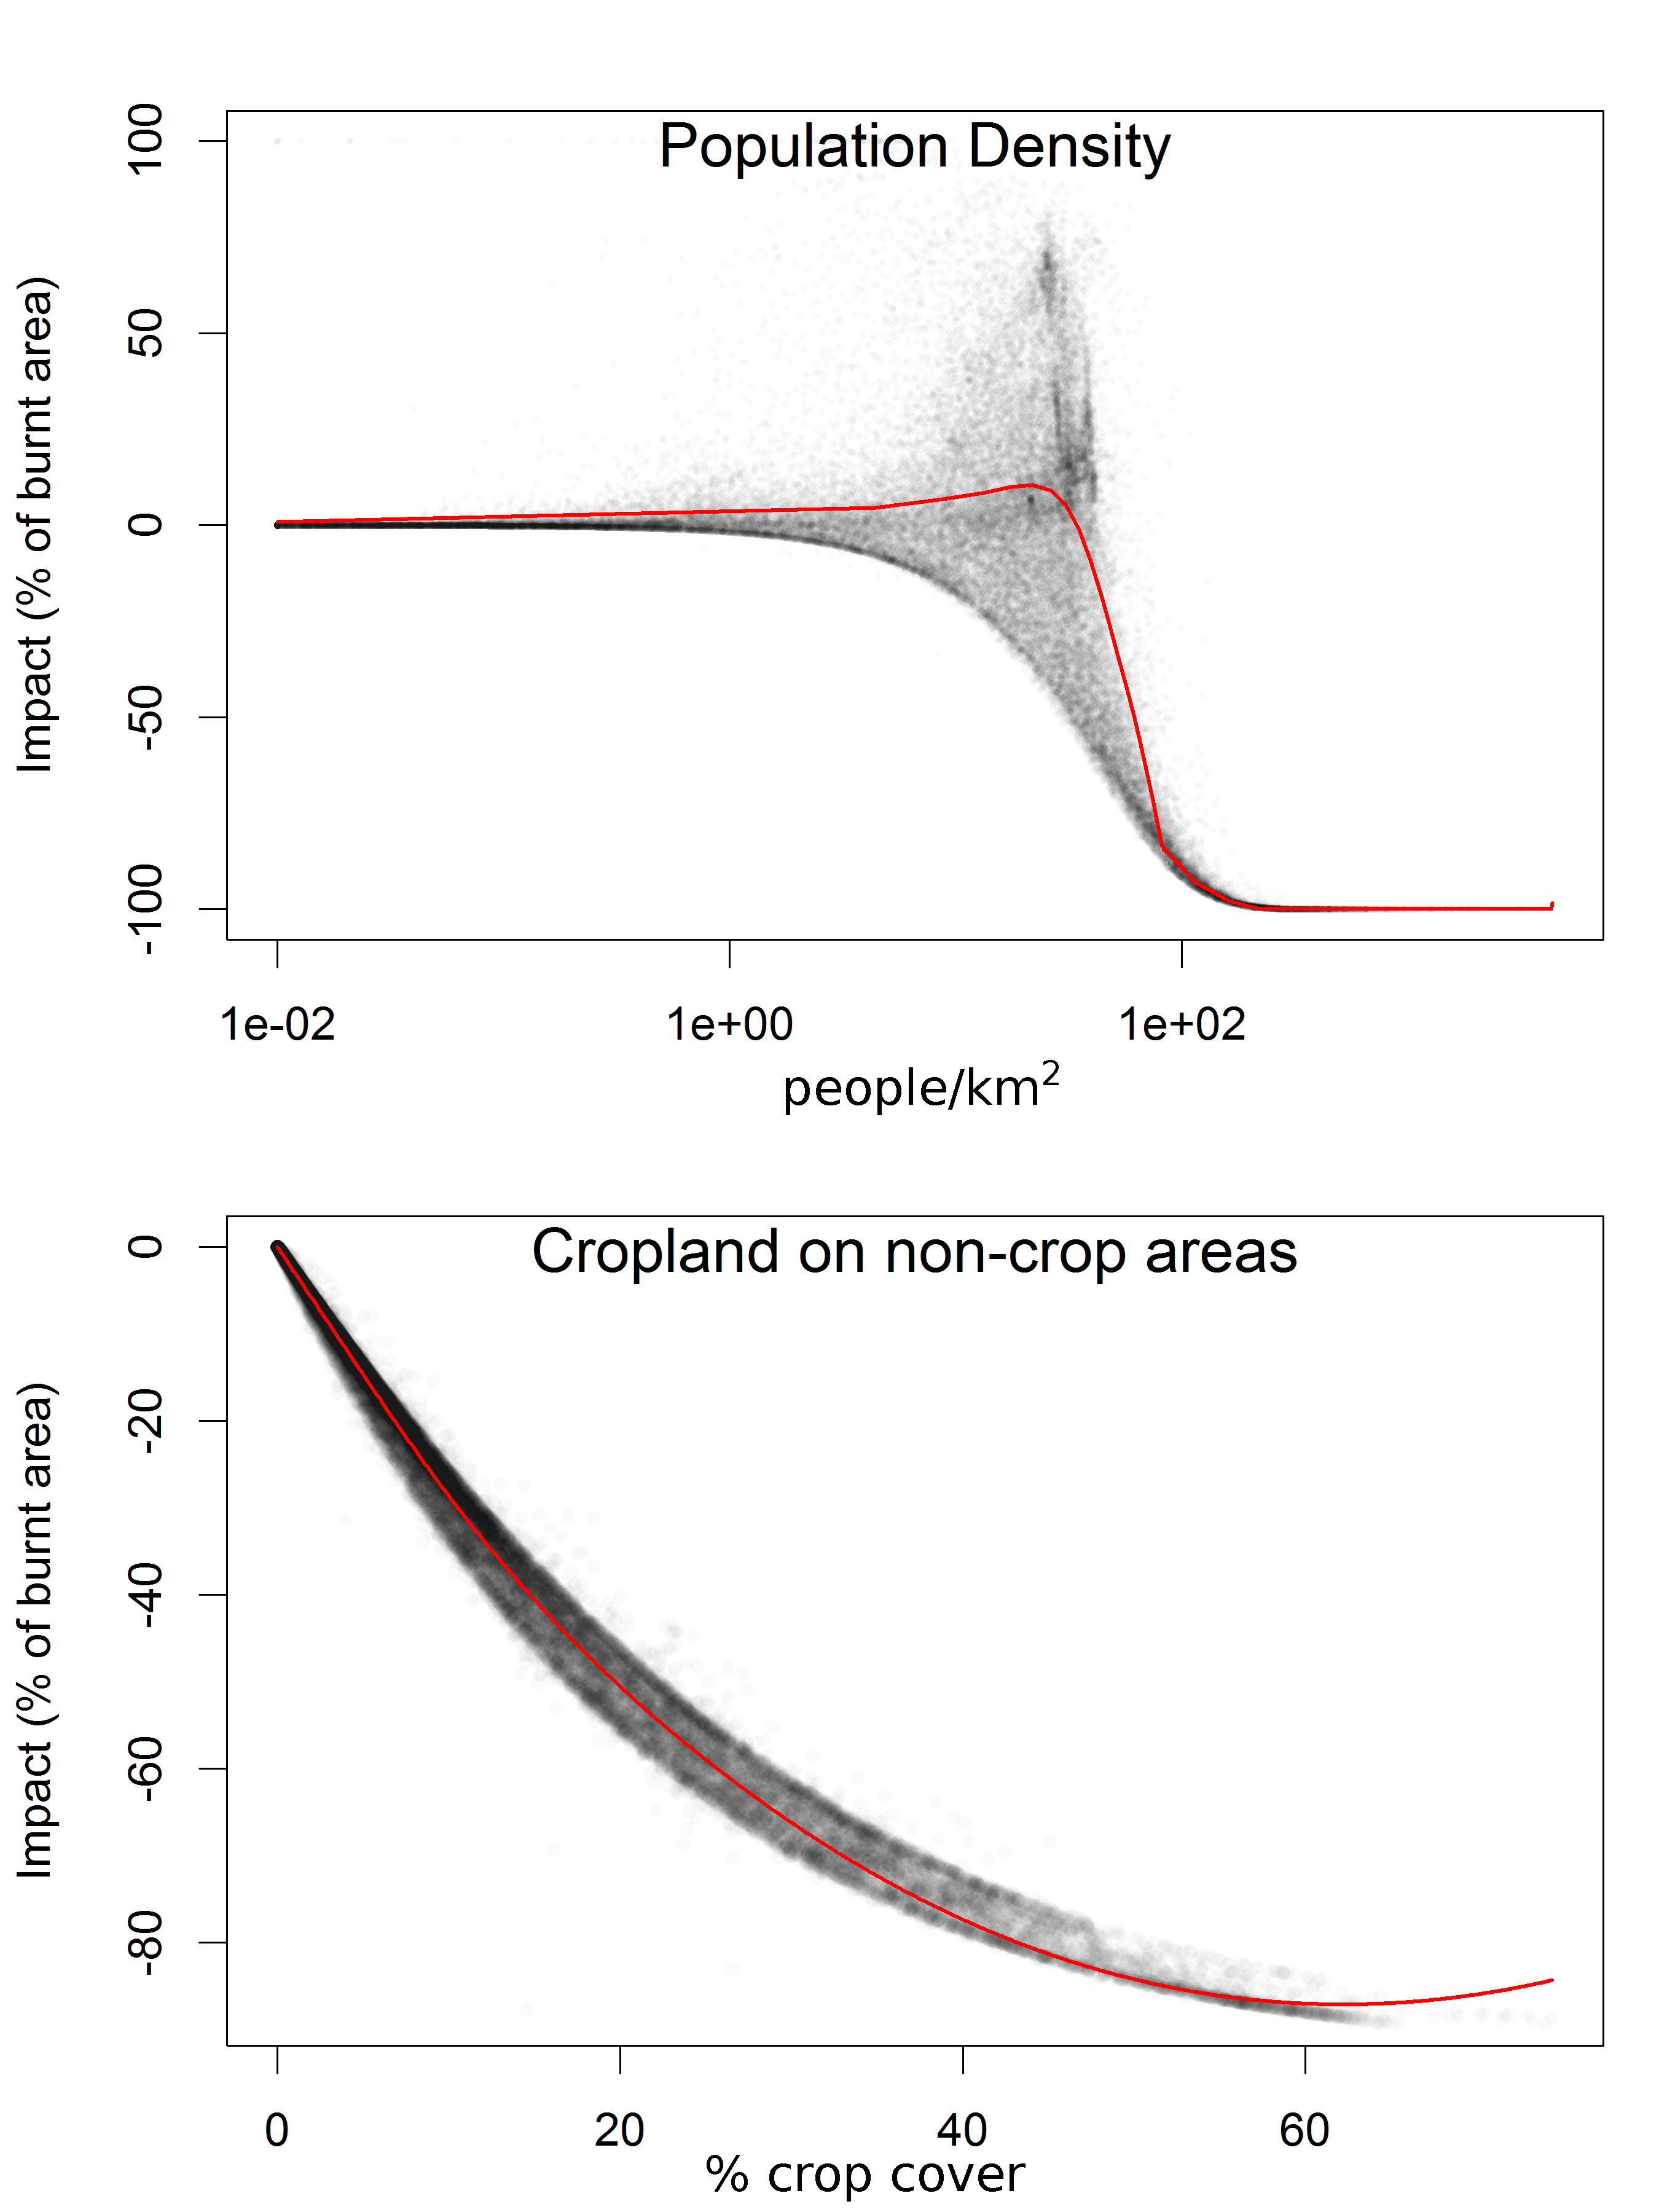
\includegraphics[width=5.5cm]{images/human_noHuman_impact}
    }
    \end{textblock*}

    %\visible<3->{
    %    \begin{tikzpicture}
    %        \node[anchor=south west,inner sep=0] (image) at (0,0) {
    %            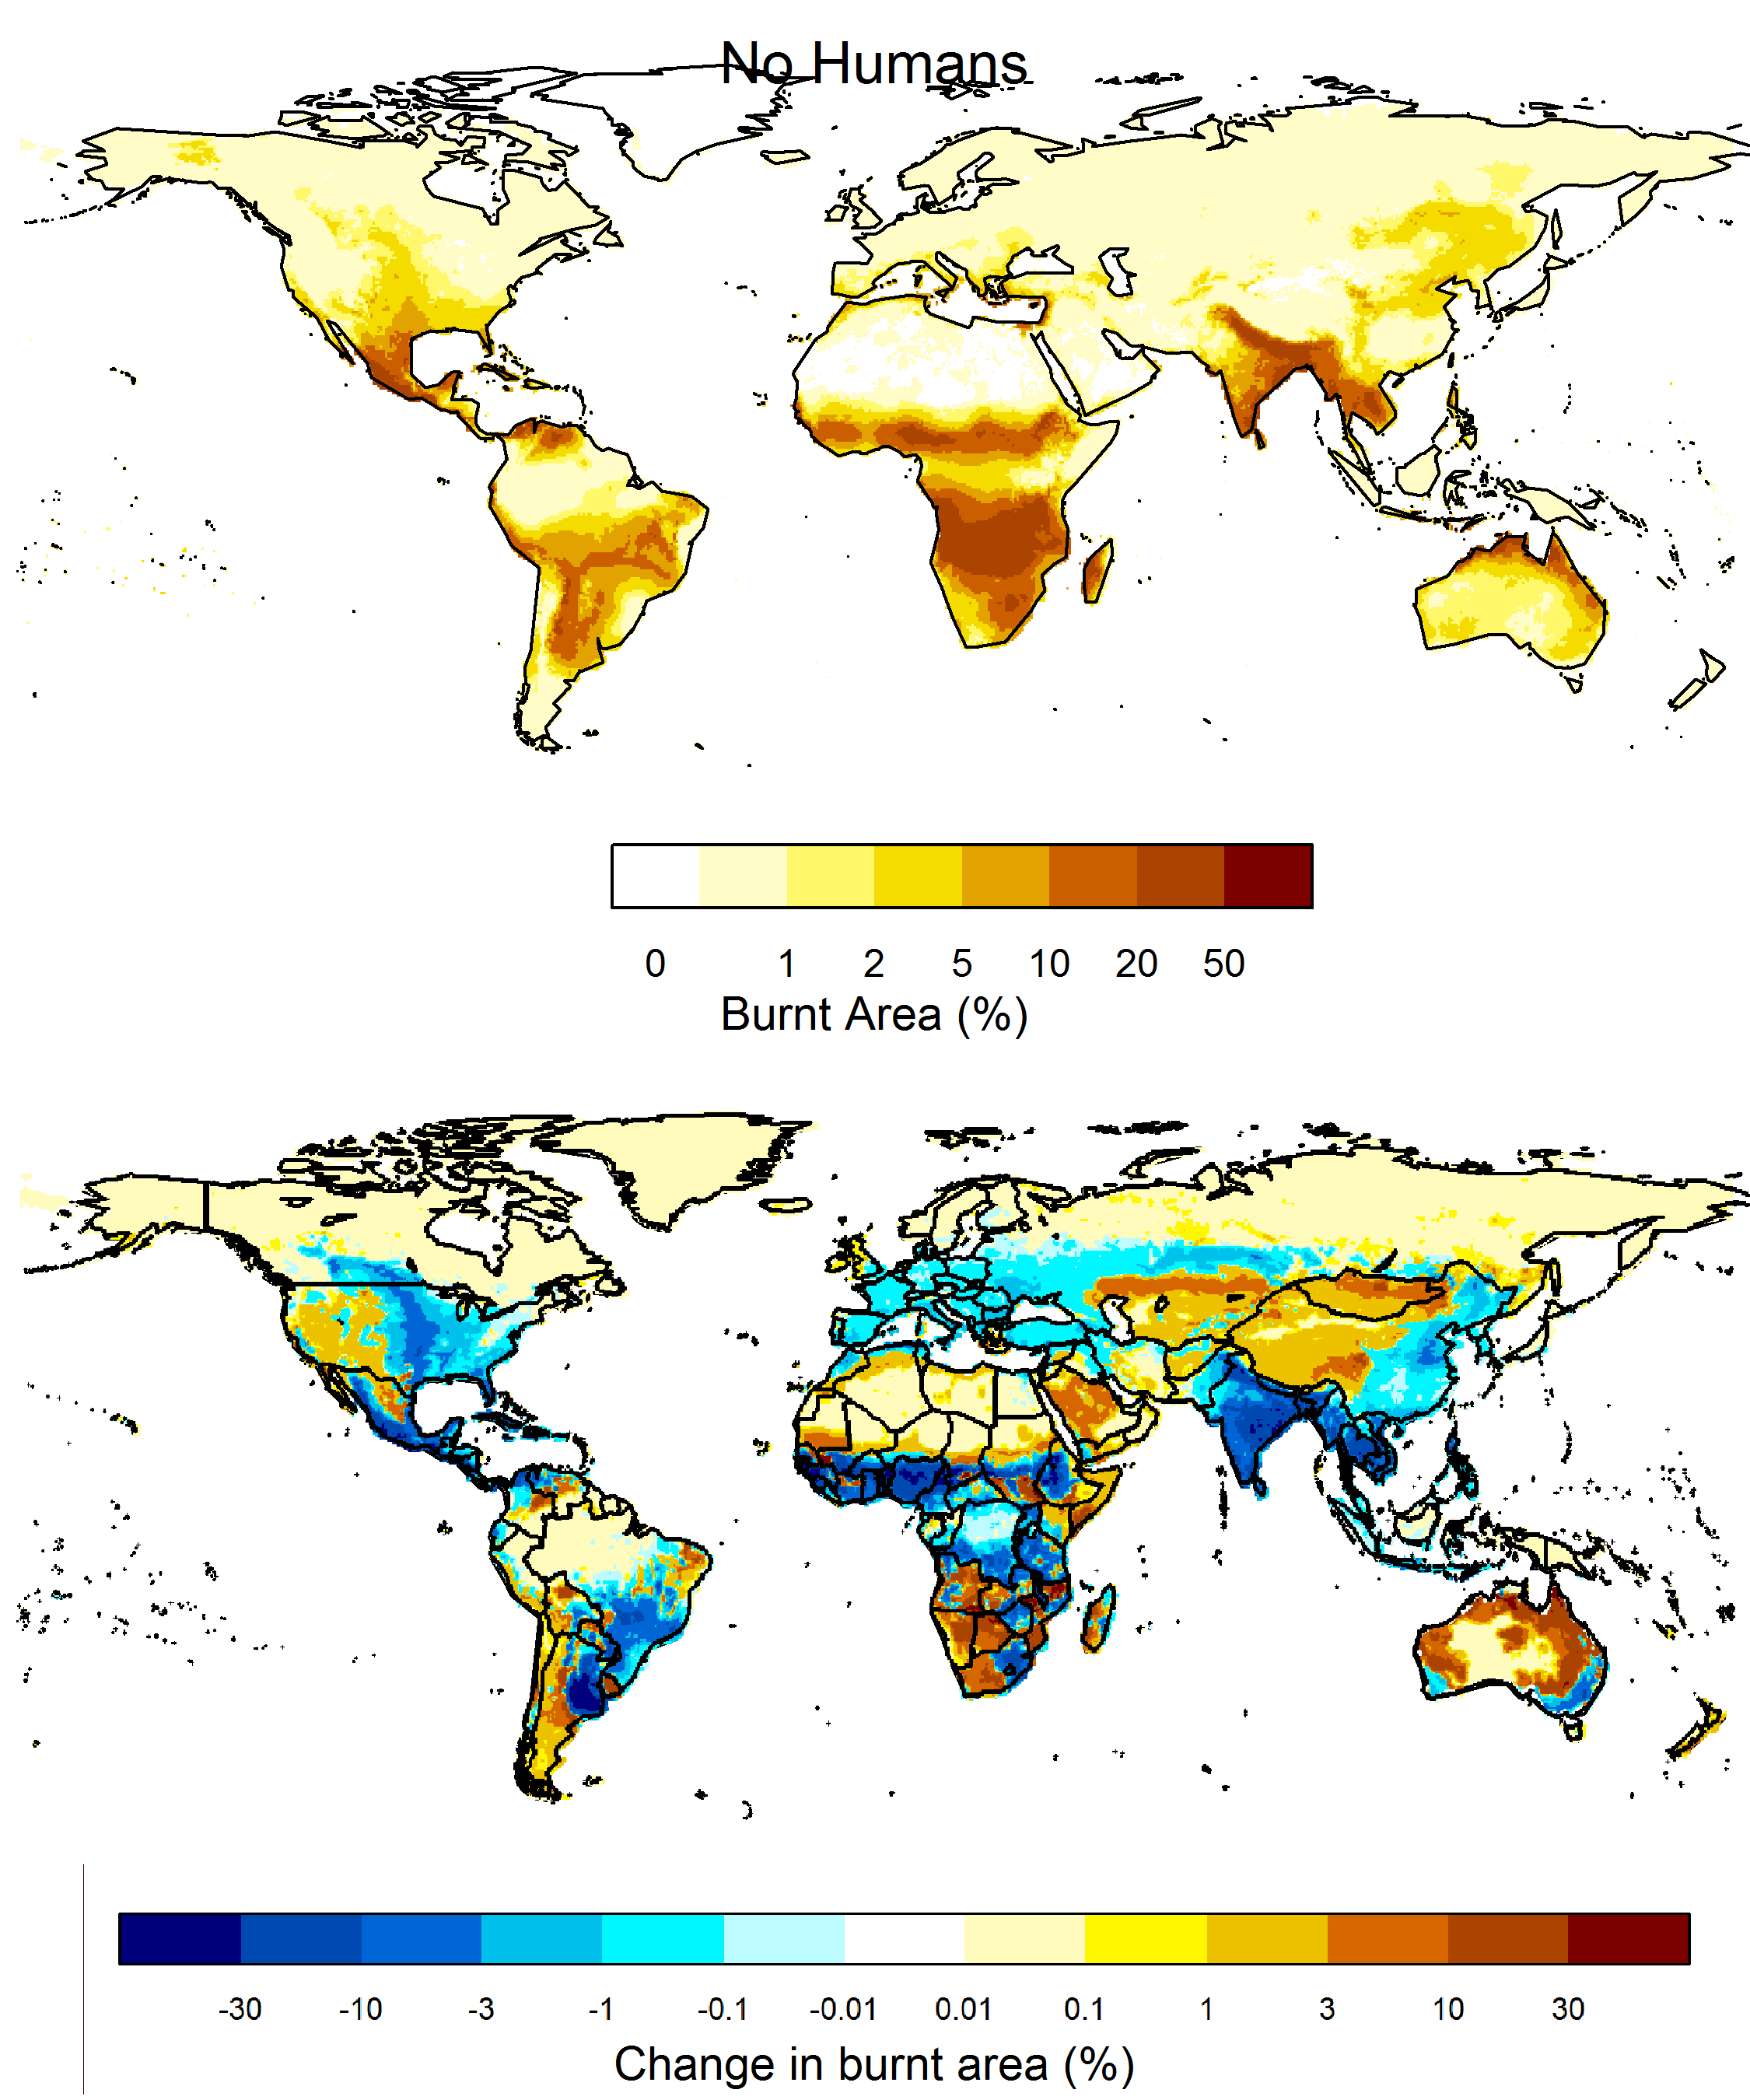
\includegraphics[trim={0 0 0 8cm},clip,width=11.0cm]{images/igntitions/IgntionInfoNoHumans}
    %        };
    %
            %\visible<-1> {\draw[white, fill = white] (5.5,4) -- (12.0,4) -- (12.0,0.0) -- (5.5,0.0) -- (5.5,4);}
    %    \end{tikzpicture}
    %}
\end{frame}

\pgfdeclareimage[width=1.0\paperwidth]{header-image}{header_images/firefighter}

%\begin{frame}<2-3>
%    \frametitle{Sensitivity to Controls}
%    \controlsSide{limitation_map}
%\end{frame}
